% =====================================================================
% Canvas3D Figure Variants Preview Document
% Compile with: xelatex preview_variants.tex
% =====================================================================
\documentclass[10pt,twocolumn]{article}

\usepackage[margin=0.8in]{geometry}
\usepackage{graphicx}
\usepackage{tikz}
\usetikzlibrary{positioning,arrows.meta,shapes.geometric,fit,calc}
\usepackage{xcolor}
\usepackage{amsmath,amssymb}
\usepackage{microtype}
\usepackage{caption}

% Compact captions for preview
\captionsetup{font={small},skip=4pt}

\begin{document}

\title{Canvas3D Figure Variants Preview}
\author{Select your preferred variant for each figure}
\date{\today}
\maketitle

\vspace{1em}
\noindent\textbf{Instructions:} Each figure below is labeled
\texttt{figX\_name\_V} where \texttt{X} is the figure number,
\texttt{name} is the module, and \texttt{V} is the variant (A/B/C).
After choosing, we will extract the corresponding code into the final
\texttt{method.tex}.

\clearpage
% =====================================================================
% Canvas3D Figure 1: Overview Pipeline - Variants A/B/C
% Layout: vertical module chain (center), inputs at top, stage labels right.
% All arrows use explicit routing, never cross any node bounding box.
% =====================================================================

% ============================ VARIANT A ==============================
\begin{figure}[t]
    \centering
    \resizebox{\linewidth}{!}{%
    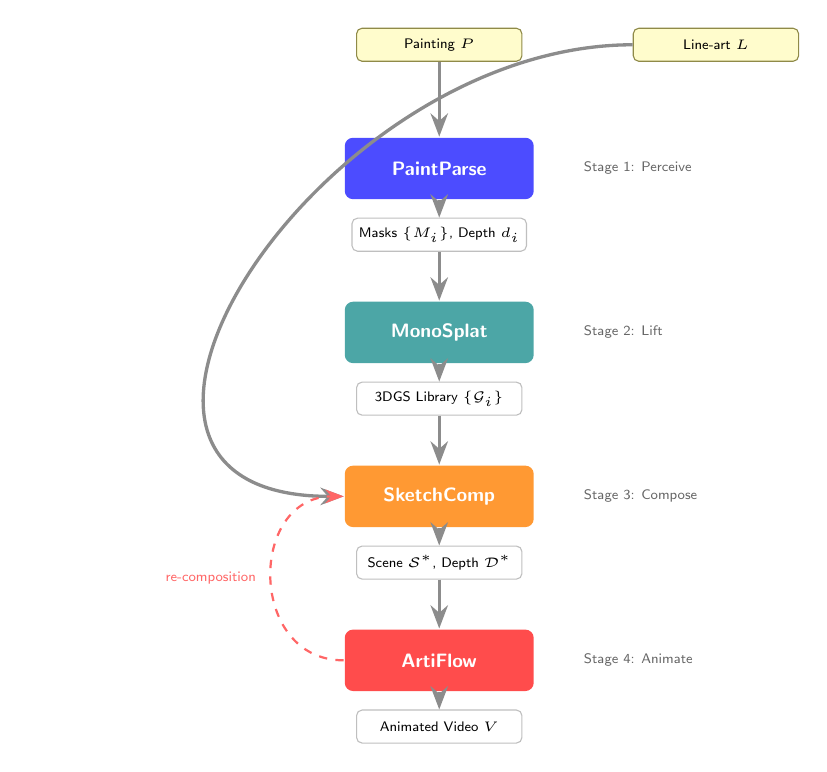
\begin{tikzpicture}[
        font=\sffamily,
        mod/.style={draw=none, rounded corners=3pt, minimum width=2.4cm,
                    minimum height=0.78cm, align=center,
                    font=\sffamily\scriptsize, text=white, thick, inner sep=3.5pt},
        data/.style={draw=black!25, rounded corners=2pt, fill=white,
                     font=\sffamily\tiny, minimum width=2.1cm,
                     minimum height=0.42cm, align=center, inner sep=2.5pt},
        lbl/.style={font=\sffamily\tiny, text=black!60},
        ar/.style={->, >=Stealth, very thick, draw=black!45},
        ar2/.style={->, >=Stealth, thick, draw=black!35, dashed}
    ]
        % --- Inputs on the top row (same baseline) ---
        \node[data, fill=yellow!20, draw=yellow!50!black] (pin) {Painting $P$};
        \node[data, fill=yellow!20, draw=yellow!50!black, right=1.4cm of pin] (lin) {Line-art $L$};

        % --- Central module chain, generous vertical gaps ---
        \node[mod, fill=blue!70,    below=0.95cm of pin] (pp)  {\textbf{PaintParse}};
        \node[data,                 below=0.22cm of pp]  (ppo) {Masks $\{M_i\}$, Depth $d_i$};
        \node[mod, fill=teal!70,    below=0.62cm of ppo] (ms)  {\textbf{MonoSplat}};
        \node[data,                 below=0.22cm of ms]  (mso) {3DGS Library $\{\mathcal{G}_i\}$};
        \node[mod, fill=orange!80,  below=0.62cm of mso] (sc)  {\textbf{SketchComp}};
        \node[data,                 below=0.22cm of sc]  (sco) {Scene $\mathcal{S}^*$, Depth $\mathcal{D}^*$};
        \node[mod, fill=red!70,     below=0.62cm of sco] (af)  {\textbf{ArtiFlow}};
        \node[data,                 below=0.22cm of af]  (afo) {Animated Video $V$};

        % --- Vertical chain: south -> north ---
        \draw[ar] (pin.south) -- (pp.north);
        \draw[ar] (pp.south)  -- (ppo.north);
        \draw[ar] (ppo.south) -- (ms.north);
        \draw[ar] (ms.south)  -- (mso.north);
        \draw[ar] (mso.south) -- (sc.north);
        \draw[ar] (sc.south)  -- (sco.north);
        \draw[ar] (sco.south) -- (af.north);
        \draw[ar] (af.south)  -- (afo.north);

        % --- Line-art to SketchComp: big left-side curve, clear of all nodes ---
        % exits west of lin, travels left on a vertical channel, enters west of sc
        \draw[ar] (lin.west) to[out=180,in=180,looseness=1.5] (sc.west);

        % --- Feedback: ArtiFlow re-composition, big left curve, dashed red ---
        \draw[ar2, draw=red!60] (af.west) to[out=180,in=180,looseness=1.5]
            node[pos=0.5, left=2pt, lbl, text=red!60, align=right] {re-composition}
            (sc.west);

        % --- Stage labels on the right column ---
        \node[lbl, right=0.5cm of pp] {Stage 1: Perceive};
        \node[lbl, right=0.5cm of ms] {Stage 2: Lift};
        \node[lbl, right=0.5cm of sc] {Stage 3: Compose};
        \node[lbl, right=0.5cm of af] {Stage 4: Animate};
    \end{tikzpicture}}
    \caption{\textbf{Canvas3D overview (Variant A).} Flat modern design with
    color-coded modules and stage annotations.}
    \label{fig:overview_A}
\end{figure}

% ============================ VARIANT B ==============================
\begin{figure}[t]
    \centering
    \resizebox{\linewidth}{!}{%
    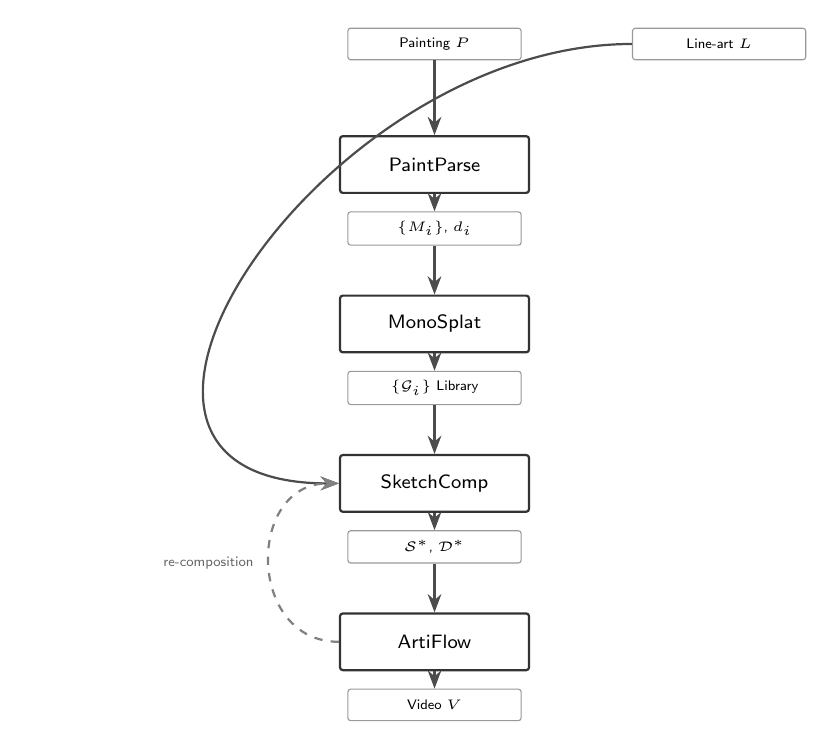
\begin{tikzpicture}[
        font=\sffamily,
        mod/.style={draw=black!80, rounded corners=1pt, minimum width=2.4cm,
                    minimum height=0.72cm, align=center,
                    font=\sffamily\scriptsize, thick},
        data/.style={draw=black!40, rounded corners=1pt, fill=white,
                     font=\sffamily\tiny, minimum width=2.2cm,
                     minimum height=0.4cm, align=center},
        ar/.style={->, >=Stealth, thick, draw=black!70},
        ar2/.style={->, >=Stealth, thick, draw=black!50, dashed}
    ]
        \node[data] (pin) {Painting $P$};
        \node[data, right=1.4cm of pin] (lin) {Line-art $L$};

        \node[mod,  below=0.95cm of pin] (pp)  {PaintParse};
        \node[data, below=0.22cm of pp]  (ppo) {$\{M_i\}$, $d_i$};
        \node[mod,  below=0.62cm of ppo] (ms)  {MonoSplat};
        \node[data, below=0.22cm of ms]  (mso) {$\{\mathcal{G}_i\}$ Library};
        \node[mod,  below=0.62cm of mso] (sc)  {SketchComp};
        \node[data, below=0.22cm of sc]  (sco) {$\mathcal{S}^*$, $\mathcal{D}^*$};
        \node[mod,  below=0.62cm of sco] (af)  {ArtiFlow};
        \node[data, below=0.22cm of af]  (afo) {Video $V$};

        \draw[ar] (pin.south) -- (pp.north);
        \draw[ar] (pp.south)  -- (ppo.north);
        \draw[ar] (ppo.south) -- (ms.north);
        \draw[ar] (ms.south)  -- (mso.north);
        \draw[ar] (mso.south) -- (sc.north);
        \draw[ar] (sc.south)  -- (sco.north);
        \draw[ar] (sco.south) -- (af.north);
        \draw[ar] (af.south)  -- (afo.north);

        \draw[ar] (lin.west) to[out=180,in=180,looseness=1.5] (sc.west);
        \draw[ar2] (af.west) to[out=180,in=180,looseness=1.5]
            node[pos=0.5, left=2pt, font=\sffamily\tiny, text=black!60, align=right]
            {re-composition} (sc.west);
    \end{tikzpicture}}
    \caption{\textbf{Canvas3D overview (Variant B).} Minimal monochrome
    line-art style, suitable for black-and-white printing.}
    \label{fig:overview_B}
\end{figure}

% ============================ VARIANT C ==============================
\begin{figure}[t]
    \centering
    \resizebox{\linewidth}{!}{%
    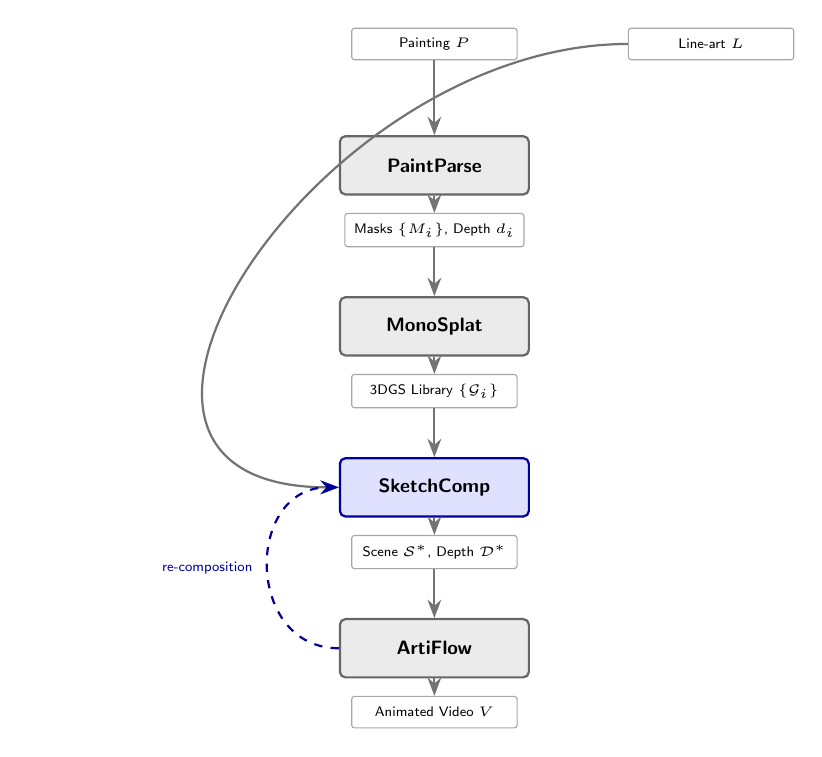
\begin{tikzpicture}[
        font=\sffamily,
        mod/.style={draw=black!60, fill=black!8, rounded corners=2pt,
                    minimum width=2.4cm, minimum height=0.74cm, align=center,
                    font=\sffamily\scriptsize, thick},
        acc/.style={draw=blue!60!black, fill=blue!12, rounded corners=2pt,
                    minimum width=2.4cm, minimum height=0.74cm, align=center,
                    font=\sffamily\scriptsize, thick},
        data/.style={draw=black!35, fill=white, rounded corners=1pt,
                     font=\sffamily\tiny, minimum width=2.1cm,
                     minimum height=0.4cm, align=center},
        ar/.style={->, >=Stealth, thick, draw=black!55},
        ar2/.style={->, >=Stealth, thick, draw=blue!60!black, dashed}
    ]
        \node[data] (pin) {Painting $P$};
        \node[data, right=1.4cm of pin] (lin) {Line-art $L$};

        \node[mod,  below=0.95cm of pin] (pp)  {\textbf{PaintParse}};
        \node[data, below=0.22cm of pp]  (ppo) {Masks $\{M_i\}$, Depth $d_i$};
        \node[mod,  below=0.62cm of ppo] (ms)  {\textbf{MonoSplat}};
        \node[data, below=0.22cm of ms]  (mso) {3DGS Library $\{\mathcal{G}_i\}$};
        \node[acc,  below=0.62cm of mso] (sc)  {\textbf{SketchComp}};
        \node[data, below=0.22cm of sc]  (sco) {Scene $\mathcal{S}^*$, Depth $\mathcal{D}^*$};
        \node[mod,  below=0.62cm of sco] (af)  {\textbf{ArtiFlow}};
        \node[data, below=0.22cm of af]  (afo) {Animated Video $V$};

        \draw[ar] (pin.south) -- (pp.north);
        \draw[ar] (pp.south)  -- (ppo.north);
        \draw[ar] (ppo.south) -- (ms.north);
        \draw[ar] (ms.south)  -- (mso.north);
        \draw[ar] (mso.south) -- (sc.north);
        \draw[ar] (sc.south)  -- (sco.north);
        \draw[ar] (sco.south) -- (af.north);
        \draw[ar] (af.south)  -- (afo.north);

        \draw[ar] (lin.west) to[out=180,in=180,looseness=1.5] (sc.west);
        \draw[ar2] (af.west) to[out=180,in=180,looseness=1.5]
            node[pos=0.5, left=2pt, font=\sffamily\tiny, text=blue!60!black, align=right]
            {re-composition} (sc.west);
    \end{tikzpicture}}
    \caption{\textbf{Canvas3D overview (Variant C).} Academic grayscale with
    blue accent highlighting the novel SketchComp module.}
    \label{fig:overview_C}
\end{figure}

\clearpage
% =====================================================================
% Canvas3D Figure 2: PaintParse - Variants A/B/C
% LAYOUT (new, collision-free):
%   pin    ->  yolo                          out
%              feat                          dm
%              head                          (then to layer, right channel)
%              dav2
%              adapt
%              layer
%   Feedback arrows from adapt back up to feat/yolo hug the LEFT side.
% =====================================================================

% ============================ VARIANT A ==============================
\begin{figure}[t]
    \centering
    \resizebox{\linewidth}{!}{%
    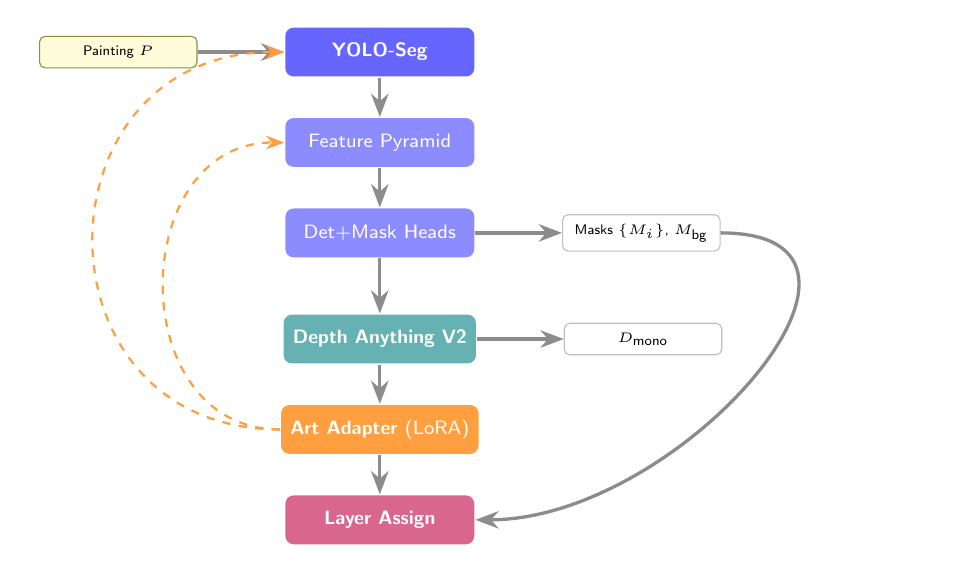
\begin{tikzpicture}[
        font=\sffamily,
        bx/.style={draw=none, rounded corners=3pt, fill=blue!60, text=white,
                   minimum width=2.4cm, minimum height=0.62cm, align=center,
                   font=\sffamily\scriptsize, thick},
        bx2/.style={draw=none, rounded corners=3pt, fill=teal!60, text=white,
                    minimum width=2.4cm, minimum height=0.62cm, align=center,
                    font=\sffamily\scriptsize, thick},
        bx3/.style={draw=none, rounded corners=3pt, fill=orange!75, text=white,
                    minimum width=2.4cm, minimum height=0.62cm, align=center,
                    font=\sffamily\scriptsize, thick},
        data/.style={draw=black!25, rounded corners=2pt, fill=white,
                     font=\sffamily\tiny, minimum width=2.0cm,
                     minimum height=0.4cm, align=center},
        ar/.style={->, >=Stealth, very thick, draw=black!45},
        ard/.style={->, >=Stealth, thick, draw=orange!75, dashed}
    ]
        % --- Input ---
        \node[data, fill=yellow!15, draw=yellow!50!black] (pin) {Painting $P$};

        % --- One central column (x aligned) ---
        \node[bx,  right=1.1cm of pin] (yolo) {\textbf{YOLO-Seg}};
        \node[bx,  below=0.5cm of yolo, fill=blue!45] (feat) {Feature Pyramid};
        \node[bx,  below=0.5cm of feat, fill=blue!45] (head) {Det+Mask Heads};
        \node[bx2, below=0.7cm of head] (dav2)
            {\textbf{Depth Anything V2}};
        \node[bx3, below=0.5cm of dav2] (adapt)
            {\textbf{Art Adapter} (LoRA)};
        \node[bx3, below=0.5cm of adapt, fill=purple!60] (layer)
            {\textbf{Layer Assign}};

        % --- Output chips on the right side of their parent ---
        \node[data, right=1.1cm of head] (out)
            {Masks $\{M_i\}$, $M_\text{bg}$};
        \node[data, right=1.1cm of dav2] (dm)  {$D_\text{mono}$};

        % --- Straight main chain (no crossings) ---
        \draw[ar] (pin.east)   -- (yolo.west);
        \draw[ar] (yolo.south) -- (feat.north);
        \draw[ar] (feat.south) -- (head.north);
        \draw[ar] (head.south) -- (dav2.north);
        \draw[ar] (dav2.south) -- (adapt.north);
        \draw[ar] (adapt.south) -- (layer.north);

        % --- Outputs ---
        \draw[ar] (head.east) -- (out.west);
        \draw[ar] (dav2.east) -- (dm.west);

        % --- out -> layer : right-side big curve, clear of dm ---
        \draw[ar] (out.east) to[out=0,in=0,looseness=1.4] (layer.east);

        % --- LoRA feedback: adapt -> feat, adapt -> yolo via LEFT channel ---
        \draw[ard] (adapt.west) to[out=180,in=180,looseness=1.4] (feat.west);
        \draw[ard] (adapt.west) to[out=180,in=180,looseness=1.7] (yolo.west);
    \end{tikzpicture}}
    \caption{\textbf{PaintParse (Variant A).} Modern flat colors: blue for
    segmentation, teal for depth, orange for art-domain adapters.}
    \label{fig:paintparse_A}
\end{figure}

% ============================ VARIANT B ==============================
\begin{figure}[t]
    \centering
    \resizebox{\linewidth}{!}{%
    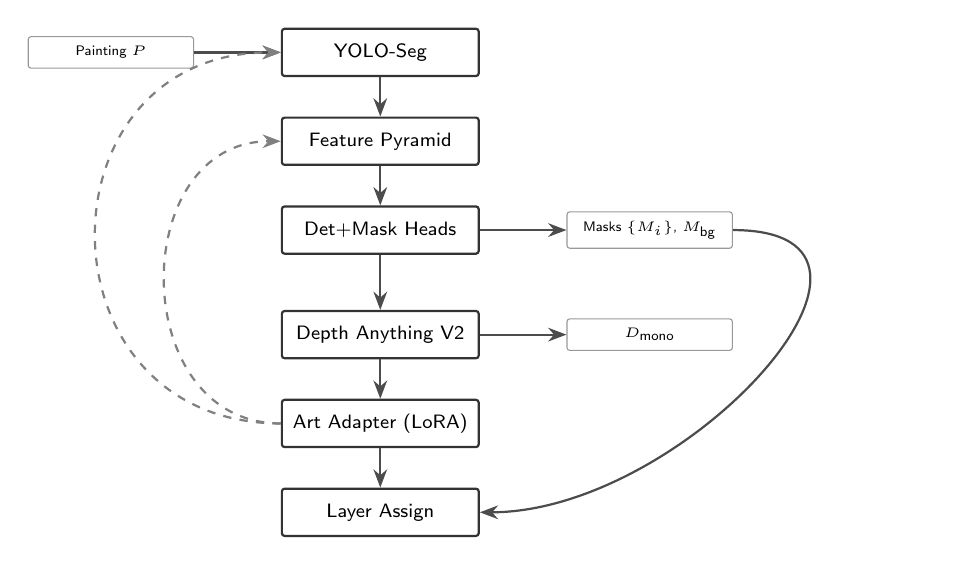
\begin{tikzpicture}[
        font=\sffamily,
        bx/.style={draw=black!80, rounded corners=1pt, minimum width=2.5cm,
                   minimum height=0.6cm, align=center,
                   font=\sffamily\scriptsize, thick},
        data/.style={draw=black!40, rounded corners=1pt, fill=white,
                     font=\sffamily\tiny, minimum width=2.1cm,
                     minimum height=0.4cm, align=center},
        ar/.style={->, >=Stealth, thick, draw=black!70},
        ard/.style={->, >=Stealth, thick, draw=black!50, dashed}
    ]
        \node[data] (pin) {Painting $P$};

        \node[bx, right=1.1cm of pin] (yolo) {YOLO-Seg};
        \node[bx, below=0.5cm of yolo] (feat) {Feature Pyramid};
        \node[bx, below=0.5cm of feat] (head) {Det+Mask Heads};
        \node[bx, below=0.7cm of head] (dav2) {Depth Anything V2};
        \node[bx, below=0.5cm of dav2] (adapt) {Art Adapter (LoRA)};
        \node[bx, below=0.5cm of adapt] (layer) {Layer Assign};

        \node[data, right=1.1cm of head] (out)
            {Masks $\{M_i\}$, $M_\text{bg}$};
        \node[data, right=1.1cm of dav2] (dm) {$D_\text{mono}$};

        \draw[ar] (pin.east)   -- (yolo.west);
        \draw[ar] (yolo.south) -- (feat.north);
        \draw[ar] (feat.south) -- (head.north);
        \draw[ar] (head.south) -- (dav2.north);
        \draw[ar] (dav2.south) -- (adapt.north);
        \draw[ar] (adapt.south) -- (layer.north);

        \draw[ar] (head.east) -- (out.west);
        \draw[ar] (dav2.east) -- (dm.west);

        \draw[ar] (out.east) to[out=0,in=0,looseness=1.4] (layer.east);

        \draw[ard] (adapt.west) to[out=180,in=180,looseness=1.4] (feat.west);
        \draw[ard] (adapt.west) to[out=180,in=180,looseness=1.7] (yolo.west);
    \end{tikzpicture}}
    \caption{\textbf{PaintParse (Variant B).} Monochrome minimal style, all
    modules white with thin outlines.}
    \label{fig:paintparse_B}
\end{figure}

% ============================ VARIANT C ==============================
\begin{figure}[t]
    \centering
    \resizebox{\linewidth}{!}{%
    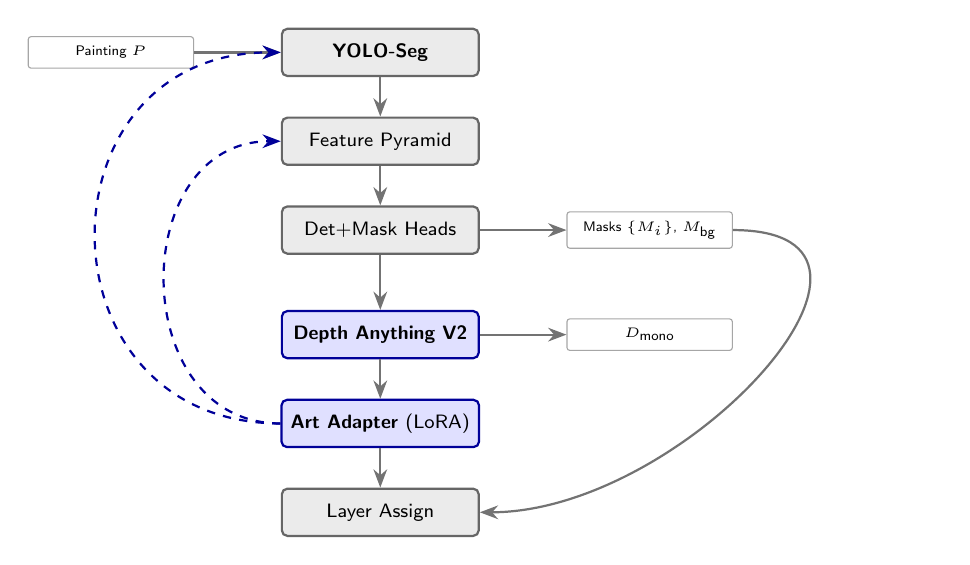
\begin{tikzpicture}[
        font=\sffamily,
        bx/.style={draw=black!60, fill=black!8, rounded corners=2pt,
                   minimum width=2.5cm, minimum height=0.6cm, align=center,
                   font=\sffamily\scriptsize, thick},
        acc/.style={draw=blue!60!black, fill=blue!12, rounded corners=2pt,
                    minimum width=2.5cm, minimum height=0.6cm, align=center,
                    font=\sffamily\scriptsize, thick},
        data/.style={draw=black!35, fill=white, rounded corners=1pt,
                     font=\sffamily\tiny, minimum width=2.1cm,
                     minimum height=0.4cm, align=center},
        ar/.style={->, >=Stealth, thick, draw=black!55},
        ard/.style={->, >=Stealth, thick, draw=blue!60!black, dashed}
    ]
        \node[data] (pin) {Painting $P$};

        \node[bx,  right=1.1cm of pin] (yolo) {\textbf{YOLO-Seg}};
        \node[bx,  below=0.5cm of yolo] (feat) {Feature Pyramid};
        \node[bx,  below=0.5cm of feat] (head) {Det+Mask Heads};
        \node[acc, below=0.7cm of head] (dav2)
            {\textbf{Depth Anything V2}};
        \node[acc, below=0.5cm of dav2] (adapt)
            {\textbf{Art Adapter} (LoRA)};
        \node[bx,  below=0.5cm of adapt] (layer) {Layer Assign};

        \node[data, right=1.1cm of head] (out)
            {Masks $\{M_i\}$, $M_\text{bg}$};
        \node[data, right=1.1cm of dav2] (dm) {$D_\text{mono}$};

        \draw[ar] (pin.east)   -- (yolo.west);
        \draw[ar] (yolo.south) -- (feat.north);
        \draw[ar] (feat.south) -- (head.north);
        \draw[ar] (head.south) -- (dav2.north);
        \draw[ar] (dav2.south) -- (adapt.north);
        \draw[ar] (adapt.south) -- (layer.north);

        \draw[ar] (head.east) -- (out.west);
        \draw[ar] (dav2.east) -- (dm.west);

        \draw[ar] (out.east) to[out=0,in=0,looseness=1.4] (layer.east);

        \draw[ard] (adapt.west) to[out=180,in=180,looseness=1.4] (feat.west);
        \draw[ard] (adapt.west) to[out=180,in=180,looseness=1.7] (yolo.west);
    \end{tikzpicture}}
    \caption{\textbf{PaintParse (Variant C).} Grayscale with blue accent on
    depth/adapter branches, emphasizing the novel art-domain adaptation.}
    \label{fig:paintparse_C}
\end{figure}

\clearpage
% =====================================================================
% Canvas3D Figure 3: MonoSplat - Variants A/B/C
% LAYOUT: crop -> tripo -> out flowing left-to-right,
%         sc (metric-rescale) sits centered BELOW tripo,
%         lib (3DGS library) sits centered BELOW out.
%   Edge routing:
%     crop.east -> tripo.west        (straight)
%     tripo.east -> out.west         (straight)
%     out.south -> lib.north         (straight, vertical drop)
%     tripo.south -> sc.north        (straight, vertical drop)
%     sc.east -> lib.west            (straight, horizontal)
%   No curves needed, no crossings.
% =====================================================================

% ============================ VARIANT A ==============================
\begin{figure}[t]
    \centering
    \resizebox{\linewidth}{!}{%
    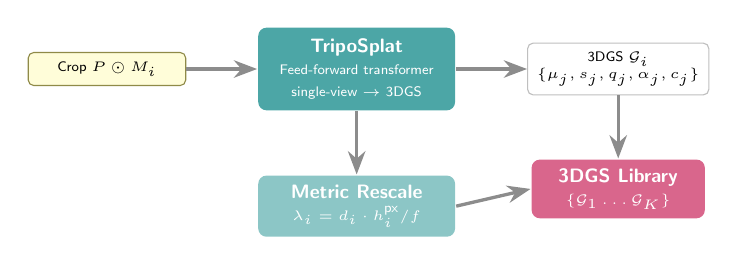
\begin{tikzpicture}[
        font=\sffamily,
        bx/.style={draw=none, rounded corners=3pt, minimum width=2.3cm,
                   minimum height=0.72cm, align=center,
                   font=\sffamily\scriptsize, thick, text=white},
        data/.style={draw=black!25, rounded corners=2pt, fill=white,
                     font=\sffamily\tiny, minimum width=2.0cm,
                     minimum height=0.42cm, align=center},
        ar/.style={->, >=Stealth, very thick, draw=black!45}
    ]
        % --- Top row: crop -> tripo -> out ---
        \node[data, fill=yellow!15, draw=yellow!50!black] (crop)
            {Crop $P \odot M_i$};
        \node[bx, fill=teal!70, right=0.9cm of crop,
              minimum width=2.5cm, minimum height=1.05cm] (tripo)
            {\textbf{TripoSplat}\\{\tiny Feed-forward transformer}\\{\tiny single-view $\to$ 3DGS}};
        \node[data, right=0.9cm of tripo] (out)
            {3DGS $\mathcal{G}_i$\\{\tiny $\{\mu_j, s_j, q_j, \alpha_j, c_j\}$}};

        % --- Bottom row, x-aligned with their parents ---
        \node[bx, fill=teal!45, below=0.8cm of tripo,
              minimum width=2.5cm] (sc)
            {\textbf{Metric Rescale}\\{\tiny $\lambda_i = d_i \cdot h_i^\text{px}/f$}};
        \node[bx, fill=purple!60, below=0.8cm of out,
              minimum width=2.2cm] (lib)
            {\textbf{3DGS Library}\\{\tiny $\{\mathcal{G}_1 \ldots \mathcal{G}_K\}$}};

        % --- All arrows are straight and collision-free ---
        \draw[ar] (crop.east)  -- (tripo.west);
        \draw[ar] (tripo.east) -- (out.west);
        \draw[ar] (tripo.south) -- (sc.north);
        \draw[ar] (out.south)   -- (lib.north);
        \draw[ar] (sc.east)     -- (lib.west);
    \end{tikzpicture}}
    \caption{\textbf{MonoSplat (Variant A).} Flat style with teal TripoSplat
    core and purple library, emphasizing the metric rescaling step.}
    \label{fig:monosplat_A}
\end{figure}

% ============================ VARIANT B ==============================
\begin{figure}[t]
    \centering
    \resizebox{\linewidth}{!}{%
    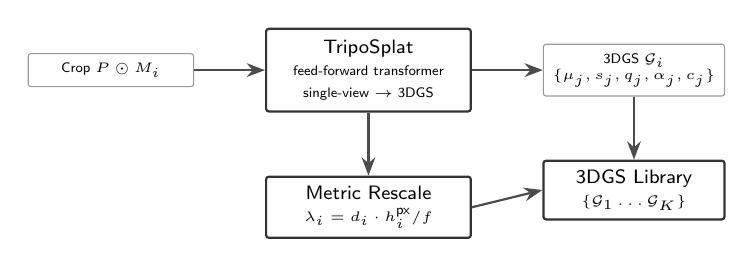
\begin{tikzpicture}[
        font=\sffamily,
        bx/.style={draw=black!80, rounded corners=1pt, minimum width=2.4cm,
                   minimum height=0.72cm, align=center,
                   font=\sffamily\scriptsize, thick},
        data/.style={draw=black!40, rounded corners=1pt, fill=white,
                     font=\sffamily\tiny, minimum width=2.1cm,
                     minimum height=0.42cm, align=center},
        ar/.style={->, >=Stealth, thick, draw=black!70}
    ]
        \node[data] (crop) {Crop $P \odot M_i$};
        \node[bx, right=0.9cm of crop, minimum width=2.6cm,
              minimum height=1.05cm] (tripo)
            {TripoSplat\\{\tiny feed-forward transformer}\\{\tiny single-view $\to$ 3DGS}};
        \node[data, right=0.9cm of tripo] (out)
            {3DGS $\mathcal{G}_i$\\{\tiny $\{\mu_j, s_j, q_j, \alpha_j, c_j\}$}};

        \node[bx, below=0.8cm of tripo, minimum width=2.6cm] (sc)
            {Metric Rescale\\{\tiny $\lambda_i = d_i \cdot h_i^\text{px}/f$}};
        \node[bx, below=0.8cm of out, minimum width=2.3cm] (lib)
            {3DGS Library\\{\tiny $\{\mathcal{G}_1 \ldots \mathcal{G}_K\}$}};

        \draw[ar] (crop.east)  -- (tripo.west);
        \draw[ar] (tripo.east) -- (out.west);
        \draw[ar] (tripo.south) -- (sc.north);
        \draw[ar] (out.south)   -- (lib.north);
        \draw[ar] (sc.east)     -- (lib.west);
    \end{tikzpicture}}
    \caption{\textbf{MonoSplat (Variant B).} Monochrome line style, no fills,
    maximum clarity for print.}
    \label{fig:monosplat_B}
\end{figure}

% ============================ VARIANT C ==============================
\begin{figure}[t]
    \centering
    \resizebox{\linewidth}{!}{%
    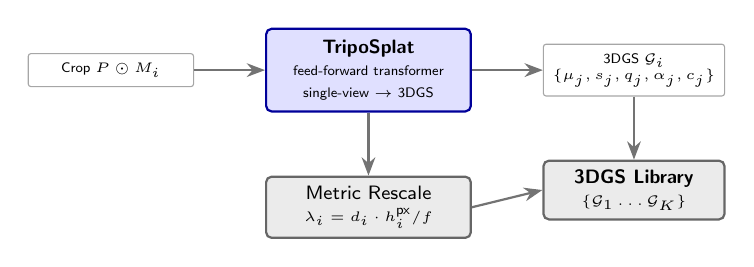
\begin{tikzpicture}[
        font=\sffamily,
        bx/.style={draw=black!60, fill=black!8, rounded corners=2pt,
                   minimum width=2.4cm, minimum height=0.72cm, align=center,
                   font=\sffamily\scriptsize, thick},
        acc/.style={draw=blue!60!black, fill=blue!12, rounded corners=2pt,
                    minimum width=2.4cm, minimum height=0.72cm, align=center,
                    font=\sffamily\scriptsize, thick},
        data/.style={draw=black!35, fill=white, rounded corners=1pt,
                     font=\sffamily\tiny, minimum width=2.1cm,
                     minimum height=0.42cm, align=center},
        ar/.style={->, >=Stealth, thick, draw=black!55}
    ]
        \node[data] (crop) {Crop $P \odot M_i$};
        \node[acc, right=0.9cm of crop, minimum width=2.6cm,
              minimum height=1.05cm] (tripo)
            {\textbf{TripoSplat}\\{\tiny feed-forward transformer}\\{\tiny single-view $\to$ 3DGS}};
        \node[data, right=0.9cm of tripo] (out)
            {3DGS $\mathcal{G}_i$\\{\tiny $\{\mu_j, s_j, q_j, \alpha_j, c_j\}$}};

        \node[bx, below=0.8cm of tripo, minimum width=2.6cm] (sc)
            {Metric Rescale\\{\tiny $\lambda_i = d_i \cdot h_i^\text{px}/f$}};
        \node[bx, below=0.8cm of out, minimum width=2.3cm] (lib)
            {\textbf{3DGS Library}\\{\tiny $\{\mathcal{G}_1 \ldots \mathcal{G}_K\}$}};

        \draw[ar] (crop.east)  -- (tripo.west);
        \draw[ar] (tripo.east) -- (out.west);
        \draw[ar] (tripo.south) -- (sc.north);
        \draw[ar] (out.south)   -- (lib.north);
        \draw[ar] (sc.east)     -- (lib.west);
    \end{tikzpicture}}
    \caption{\textbf{MonoSplat (Variant C).} Grayscale with blue accent on
    the core TripoSplat module, Gaussian parameterization visible.}
    \label{fig:monosplat_C}
\end{figure}

\clearpage
% =====================================================================
% Canvas3D Figure 4: SketchComp - Variants A/B/C
% LAYOUT (new, collision-free, clean):
%   Row 0 (top):    [la]        [lib]
%   Row 1:                       [match]        [plc]
%   Row 2:                       [comp]         [gap]
%   Row 3:                       [inp]          [fin]
%
%   Straight vertical column match -> comp -> inp (the pipeline),
%   Inputs la (to match) and lib (to match) enter from the west.
%   plc / gap / fin are output chips, sitting to the right of their producer.
%   Right-side route: plc -> comp (down), comp -> gap, gap -> inp, inp -> fin.
% =====================================================================

% ============================ VARIANT A ==============================
\begin{figure}[t]
    \centering
    \resizebox{\linewidth}{!}{%
    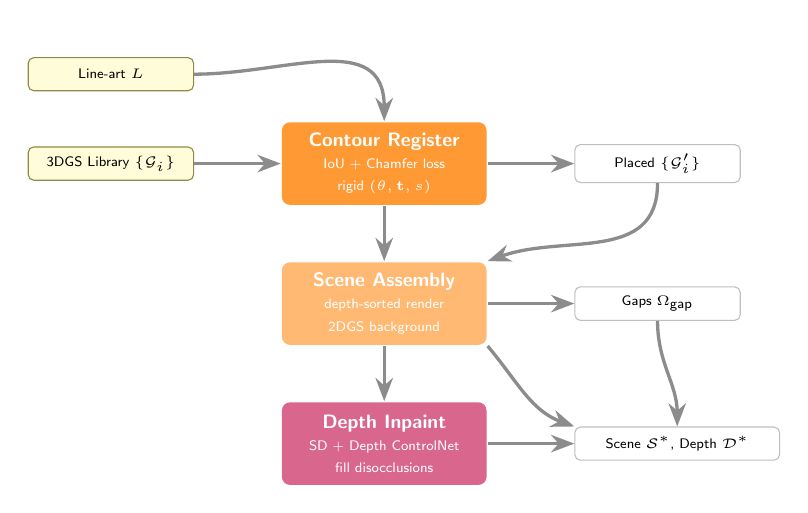
\begin{tikzpicture}[
        font=\sffamily,
        bx/.style={draw=none, rounded corners=3pt, minimum width=2.5cm,
                   minimum height=0.72cm, align=center,
                   font=\sffamily\scriptsize, thick, text=white},
        data/.style={draw=black!25, rounded corners=2pt, fill=white,
                     font=\sffamily\tiny, minimum width=2.1cm,
                     minimum height=0.42cm, align=center},
        ar/.style={->, >=Stealth, very thick, draw=black!45}
    ]
        % --- Inputs ---
        \node[data, fill=yellow!15, draw=yellow!50!black] (la) {Line-art $L$};
        \node[data, fill=yellow!15, draw=yellow!50!black, below=0.7cm of la] (lib)
            {3DGS Library $\{\mathcal{G}_i\}$};

        % --- Center pipeline column ---
        \node[bx, fill=orange!80, right=1.1cm of lib,
              minimum width=2.6cm, minimum height=1.05cm] (match)
            {\textbf{Contour Register}\\{\tiny IoU + Chamfer loss}\\{\tiny rigid $(\theta, \mathbf{t}, s)$}};
        \node[bx, fill=orange!55, below=0.7cm of match,
              minimum width=2.6cm, minimum height=1.05cm] (comp)
            {\textbf{Scene Assembly}\\{\tiny depth-sorted render}\\{\tiny 2DGS background}};
        \node[bx, fill=purple!60, below=0.7cm of comp,
              minimum width=2.6cm, minimum height=1.05cm] (inp)
            {\textbf{Depth Inpaint}\\{\tiny SD + Depth ControlNet}\\{\tiny fill disocclusions}};

        % --- Right-side outputs, aligned with their producing module ---
        \node[data, right=1.1cm of match] (plc) {Placed $\{\mathcal{G}'_i\}$};
        \node[data, right=1.1cm of comp]  (gap) {Gaps $\Omega_\text{gap}$};
        \node[data, right=1.1cm of inp, minimum width=2.6cm] (fin)
            {Scene $\mathcal{S}^*$, Depth $\mathcal{D}^*$};

        % --- Input arrows ---
        \draw[ar] (la.east)  to[out=0,in=90,looseness=1.2] (match.north);
        \draw[ar] (lib.east) -- (match.west);

        % --- Vertical pipeline ---
        \draw[ar] (match.south) -- (comp.north);
        \draw[ar] (comp.south)   -- (inp.north);

        % --- Output taps ---
        \draw[ar] (match.east) -- (plc.west);
        \draw[ar] (comp.east)  -- (gap.west);
        \draw[ar] (inp.east)   -- (fin.west);

        % --- plc -> comp (placed gaussians feed into scene assembly) ---
        \draw[ar] (plc.south) to[out=-90,in=20,looseness=1.1] (comp.north east);

        % --- gap -> inp (detected gaps drive inpainting) ---
        \draw[ar] (gap.south) to[out=-90,in=90,looseness=1.0] (fin.north);

        % --- comp -> fin (assembled scene bypass), a small right-side curve ---
        \draw[ar] (comp.south east) to[out=-50,in=160,looseness=1.0] (fin.north west);
    \end{tikzpicture}}
    \caption{\textbf{SketchComp (Variant A).} Flat colors: orange for
    registration/assembly, purple for inpainting, emphasizing the two-stage
    compose-then-fill process.}
    \label{fig:sketchcomp_A}
\end{figure}

% ============================ VARIANT B ==============================
\begin{figure}[t]
    \centering
    \resizebox{\linewidth}{!}{%
    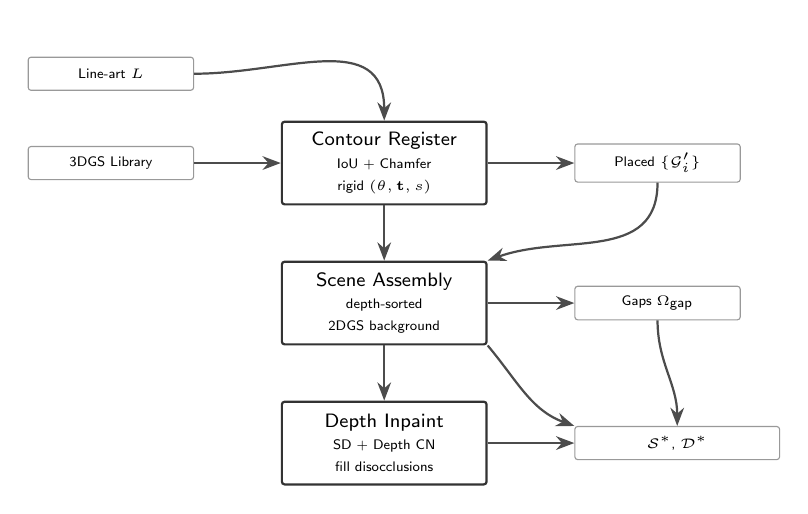
\begin{tikzpicture}[
        font=\sffamily,
        bx/.style={draw=black!80, rounded corners=1pt, minimum width=2.6cm,
                   minimum height=0.72cm, align=center,
                   font=\sffamily\scriptsize, thick},
        data/.style={draw=black!40, rounded corners=1pt, fill=white,
                     font=\sffamily\tiny, minimum width=2.1cm,
                     minimum height=0.42cm, align=center},
        ar/.style={->, >=Stealth, thick, draw=black!70}
    ]
        \node[data] (la) {Line-art $L$};
        \node[data, below=0.7cm of la] (lib) {3DGS Library};

        \node[bx, right=1.1cm of lib, minimum width=2.6cm,
              minimum height=1.05cm] (match)
            {Contour Register\\{\tiny IoU + Chamfer}\\{\tiny rigid $(\theta, \mathbf{t}, s)$}};
        \node[bx, below=0.7cm of match, minimum width=2.6cm,
              minimum height=1.05cm] (comp)
            {Scene Assembly\\{\tiny depth-sorted}\\{\tiny 2DGS background}};
        \node[bx, below=0.7cm of comp, minimum width=2.6cm,
              minimum height=1.05cm] (inp)
            {Depth Inpaint\\{\tiny SD + Depth CN}\\{\tiny fill disocclusions}};

        \node[data, right=1.1cm of match] (plc) {Placed $\{\mathcal{G}'_i\}$};
        \node[data, right=1.1cm of comp]  (gap) {Gaps $\Omega_\text{gap}$};
        \node[data, right=1.1cm of inp, minimum width=2.6cm] (fin)
            {$\mathcal{S}^*$, $\mathcal{D}^*$};

        \draw[ar] (la.east)  to[out=0,in=90,looseness=1.2] (match.north);
        \draw[ar] (lib.east) -- (match.west);
        \draw[ar] (match.south) -- (comp.north);
        \draw[ar] (comp.south)   -- (inp.north);
        \draw[ar] (match.east) -- (plc.west);
        \draw[ar] (comp.east)  -- (gap.west);
        \draw[ar] (inp.east)   -- (fin.west);
        \draw[ar] (plc.south) to[out=-90,in=20,looseness=1.1] (comp.north east);
        \draw[ar] (gap.south) to[out=-90,in=90,looseness=1.0] (fin.north);
        \draw[ar] (comp.south east) to[out=-50,in=160,looseness=1.0] (fin.north west);
    \end{tikzpicture}}
    \caption{\textbf{SketchComp (Variant B).} Monochrome line style, no fills,
    maximum clarity.}
    \label{fig:sketchcomp_B}
\end{figure}

% ============================ VARIANT C ==============================
\begin{figure}[t]
    \centering
    \resizebox{\linewidth}{!}{%
    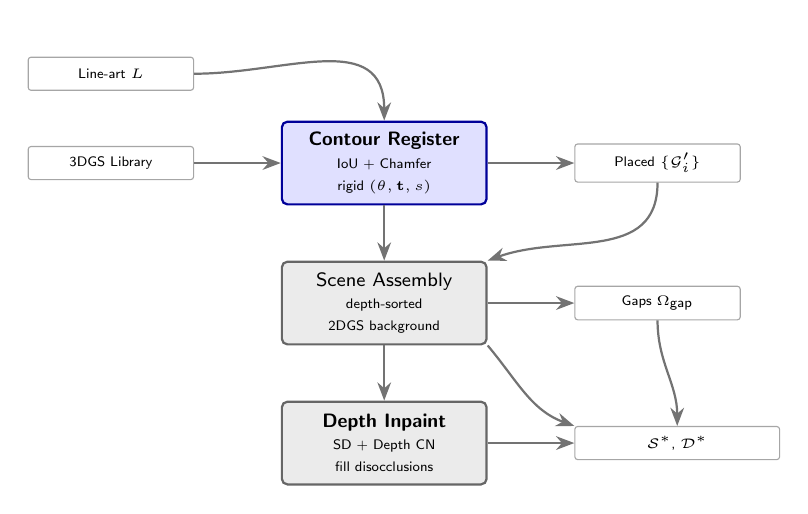
\begin{tikzpicture}[
        font=\sffamily,
        bx/.style={draw=black!60, fill=black!8, rounded corners=2pt,
                   minimum width=2.6cm, minimum height=0.72cm, align=center,
                   font=\sffamily\scriptsize, thick},
        acc/.style={draw=blue!60!black, fill=blue!12, rounded corners=2pt,
                    minimum width=2.6cm, minimum height=0.72cm, align=center,
                    font=\sffamily\scriptsize, thick},
        data/.style={draw=black!35, fill=white, rounded corners=1pt,
                     font=\sffamily\tiny, minimum width=2.1cm,
                     minimum height=0.42cm, align=center},
        ar/.style={->, >=Stealth, thick, draw=black!55}
    ]
        \node[data] (la) {Line-art $L$};
        \node[data, below=0.7cm of la] (lib) {3DGS Library};

        \node[acc, right=1.1cm of lib, minimum width=2.6cm,
              minimum height=1.05cm] (match)
            {\textbf{Contour Register}\\{\tiny IoU + Chamfer}\\{\tiny rigid $(\theta, \mathbf{t}, s)$}};
        \node[bx, below=0.7cm of match, minimum width=2.6cm,
              minimum height=1.05cm] (comp)
            {Scene Assembly\\{\tiny depth-sorted}\\{\tiny 2DGS background}};
        \node[bx, below=0.7cm of comp, minimum width=2.6cm,
              minimum height=1.05cm] (inp)
            {\textbf{Depth Inpaint}\\{\tiny SD + Depth CN}\\{\tiny fill disocclusions}};

        \node[data, right=1.1cm of match] (plc) {Placed $\{\mathcal{G}'_i\}$};
        \node[data, right=1.1cm of comp]  (gap) {Gaps $\Omega_\text{gap}$};
        \node[data, right=1.1cm of inp, minimum width=2.6cm] (fin)
            {$\mathcal{S}^*$, $\mathcal{D}^*$};

        \draw[ar] (la.east)  to[out=0,in=90,looseness=1.2] (match.north);
        \draw[ar] (lib.east) -- (match.west);
        \draw[ar] (match.south) -- (comp.north);
        \draw[ar] (comp.south)   -- (inp.north);
        \draw[ar] (match.east) -- (plc.west);
        \draw[ar] (comp.east)  -- (gap.west);
        \draw[ar] (inp.east)   -- (fin.west);
        \draw[ar] (plc.south) to[out=-90,in=20,looseness=1.1] (comp.north east);
        \draw[ar] (gap.south) to[out=-90,in=90,looseness=1.0] (fin.north);
        \draw[ar] (comp.south east) to[out=-50,in=160,looseness=1.0] (fin.north west);
    \end{tikzpicture}}
    \caption{\textbf{SketchComp (Variant C).} Grayscale with blue accent on
    the novel contour-registration module, highlighting the contribution.}
    \label{fig:sketchcomp_C}
\end{figure}

\clearpage
% =====================================================================
% Canvas3D Figure 5: ArtiFlow - Variants A/B/C  (LAYOUT v3, collision-free)
%
% Geometry summary (all three variants share the SAME layout):
%
%       [sc]x --> [rend] --> [fr] --> [vd]  --> [out] (down)
%                  |    \--> [df]
%                  |    \--> [ef]
%                  v
%                 [cn]  (a full row below rend, x-aligned with rend)
%
% Key invariants kept by construction:
%   * vd sits on the TOP row (right of fr), never in the same vertical
%     band as df/ef/cn.
%   * cn sits on the BOTTOM row directly below rend, with a clear
%     vertical gutter between the rend column and the df/ef column.
%   * df and ef bleed down and left into cn through that gutter,
%     without touching rend, vd, or each other.
%   * fr attaches to vd via a straight east-west arrow; no big arcs.
% =====================================================================

% ============================ VARIANT A ==============================
\begin{figure}[t]
    \centering
    \resizebox{\linewidth}{!}{%
    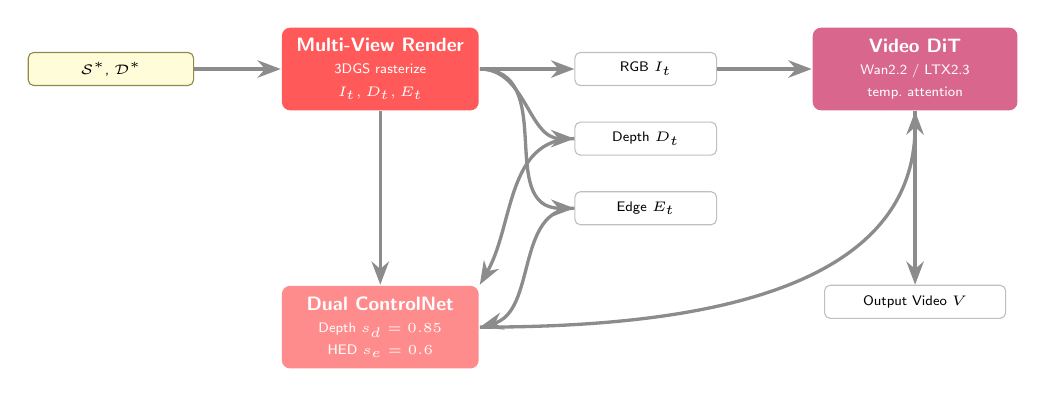
\begin{tikzpicture}[
        font=\sffamily,
        bx/.style={draw=none, rounded corners=3pt, minimum width=2.4cm,
                   minimum height=0.72cm, align=center,
                   font=\sffamily\scriptsize, thick, text=white},
        data/.style={draw=black!25, rounded corners=2pt, fill=white,
                     font=\sffamily\tiny, minimum width=2.1cm,
                     minimum height=0.42cm, align=center},
        ar/.style={->, >=Stealth, very thick, draw=black!45}
    ]
        % --- Input ---
        \node[data, fill=yellow!15, draw=yellow!50!black] (sc)
            {$\mathcal{S}^*$, $\mathcal{D}^*$};

        % --- Renderer ---
        \node[bx, fill=red!65, right=1.1cm of sc,
              minimum width=2.5cm, minimum height=1.05cm] (rend)
            {\textbf{Multi-View Render}\\{\tiny 3DGS rasterize}\\{\tiny $I_t, D_t, E_t$}};

        % --- Render products stack on rend's right ---
        \node[data, right=1.2cm of rend, minimum width=1.8cm] (fr) {RGB $I_t$};
        \node[data, below=0.45cm of fr,   minimum width=1.8cm] (df) {Depth $D_t$};
        \node[data, below=0.45cm of df,   minimum width=1.8cm] (ef) {Edge $E_t$};

        % --- ControlNet sits a FULL row below rend, x-aligned. ---
        \node[bx, fill=red!45, below=2.2cm of rend,
              minimum width=2.5cm, minimum height=1.05cm] (cn)
            {\textbf{Dual ControlNet}\\{\tiny Depth $s_d=0.85$}\\{\tiny HED $s_e=0.6$}};

        % --- Video DiT on the top row (right of fr), same baseline as rend. ---
        \node[bx, fill=purple!60, right=1.2cm of fr,
              minimum width=2.6cm, minimum height=1.05cm] (vd)
            {\textbf{Video DiT}\\{\tiny Wan2.2 / LTX2.3}\\{\tiny temp.\ attention}};

        % --- Final output below vd, but first we place an invisible anchor
        %     half a row down so `out` sits clearly under vd. ---
        \node[data, below=2.2cm of vd, minimum width=2.3cm] (out)
            {Output Video $V$};

        % ================= EDGES =================
        % Top row: straight east-west arrows.
        \draw[ar] (sc.east)   -- (rend.west);
        \draw[ar] (rend.east) -- (fr.west);
        \draw[ar] (rend.east) to[out=0,in=180,looseness=1.0] (df.west);
        \draw[ar] (rend.east) to[out=0,in=180,looseness=1.2] (ef.west);
        \draw[ar] (fr.east)   -- (vd.west);

        % Straight vertical drop from rend to cn: nothing sits in between.
        \draw[ar] (rend.south) -- (cn.north);

        % df -> cn: down-left diagonal inside the empty gutter between the
        % rend column and the df column.
        \draw[ar] (df.west) to[out=180,in=60,looseness=1.0] (cn.north east);

        % ef -> cn: drop down in the gutter to the level of cn and come in
        % from the EAST, so it never crosses vd (vd is on the top row).
        \draw[ar] (ef.west) to[out=180,in=15,looseness=1.0] (cn.east);

        % cn -> vd: gentle rising diagonal into vd.south, through the empty
        % space between the cn row and the df/ef stack.
        \draw[ar] (cn.east) to[out=0,in=-90,looseness=1.0] (vd.south);

        % vd -> out : straight vertical drop (out is directly below vd).
        \draw[ar] (vd.south) -- (out.north);
    \end{tikzpicture}}
    \caption{\textbf{ArtiFlow (Variant A).} Flat style with red for rendering,
    darker red for ControlNet, purple for the diffusion model.}
    \label{fig:artiflow_A}
\end{figure}

% ============================ VARIANT B ==============================
\begin{figure}[t]
    \centering
    \resizebox{\linewidth}{!}{%
    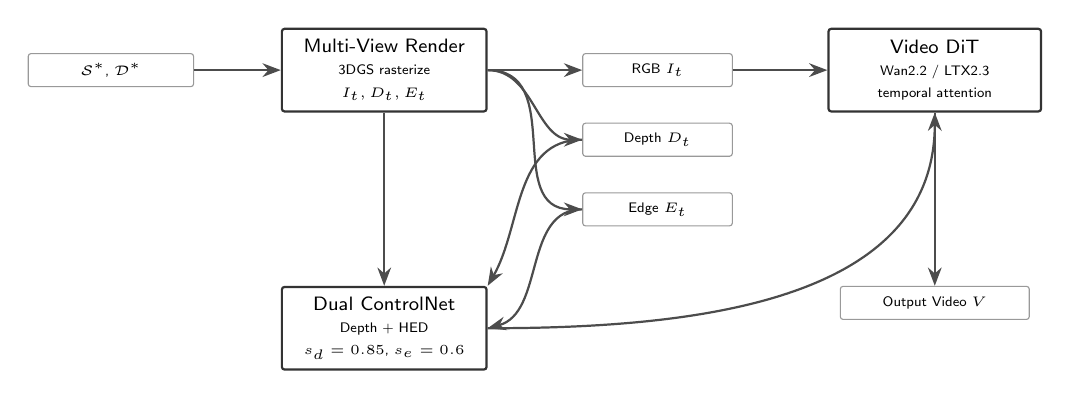
\begin{tikzpicture}[
        font=\sffamily,
        bx/.style={draw=black!80, rounded corners=1pt, minimum width=2.5cm,
                   minimum height=0.72cm, align=center,
                   font=\sffamily\scriptsize, thick},
        data/.style={draw=black!40, rounded corners=1pt, fill=white,
                     font=\sffamily\tiny, minimum width=2.1cm,
                     minimum height=0.42cm, align=center},
        ar/.style={->, >=Stealth, thick, draw=black!70}
    ]
        \node[data] (sc) {$\mathcal{S}^*$, $\mathcal{D}^*$};

        \node[bx, right=1.1cm of sc, minimum width=2.6cm,
              minimum height=1.05cm] (rend)
            {Multi-View Render\\{\tiny 3DGS rasterize}\\{\tiny $I_t, D_t, E_t$}};

        \node[data, right=1.2cm of rend, minimum width=1.9cm] (fr) {RGB $I_t$};
        \node[data, below=0.45cm of fr,   minimum width=1.9cm] (df) {Depth $D_t$};
        \node[data, below=0.45cm of df,   minimum width=1.9cm] (ef) {Edge $E_t$};

        \node[bx, below=2.2cm of rend, minimum width=2.6cm,
              minimum height=1.05cm] (cn)
            {Dual ControlNet\\{\tiny Depth + HED}\\{\tiny $s_d=0.85$, $s_e=0.6$}};

        \node[bx, right=1.2cm of fr, minimum width=2.7cm,
              minimum height=1.05cm] (vd)
            {Video DiT\\{\tiny Wan2.2 / LTX2.3}\\{\tiny temporal attention}};

        \node[data, below=2.2cm of vd, minimum width=2.4cm] (out)
            {Output Video $V$};

        \draw[ar] (sc.east)   -- (rend.west);
        \draw[ar] (rend.east) -- (fr.west);
        \draw[ar] (rend.east) to[out=0,in=180,looseness=1.0] (df.west);
        \draw[ar] (rend.east) to[out=0,in=180,looseness=1.2] (ef.west);
        \draw[ar] (fr.east)   -- (vd.west);

        \draw[ar] (rend.south) -- (cn.north);
        \draw[ar] (df.west) to[out=180,in=60,looseness=1.0] (cn.north east);
        \draw[ar] (ef.west) to[out=180,in=15,looseness=1.0] (cn.east);

        \draw[ar] (cn.east) to[out=0,in=-90,looseness=1.0] (vd.south);
        \draw[ar] (vd.south) -- (out.north);
    \end{tikzpicture}}
    \caption{\textbf{ArtiFlow (Variant B).} Monochrome line style, no fills,
    maximum clarity.}
    \label{fig:artiflow_B}
\end{figure}

% ============================ VARIANT C ==============================
\begin{figure}[t]
    \centering
    \resizebox{\linewidth}{!}{%
    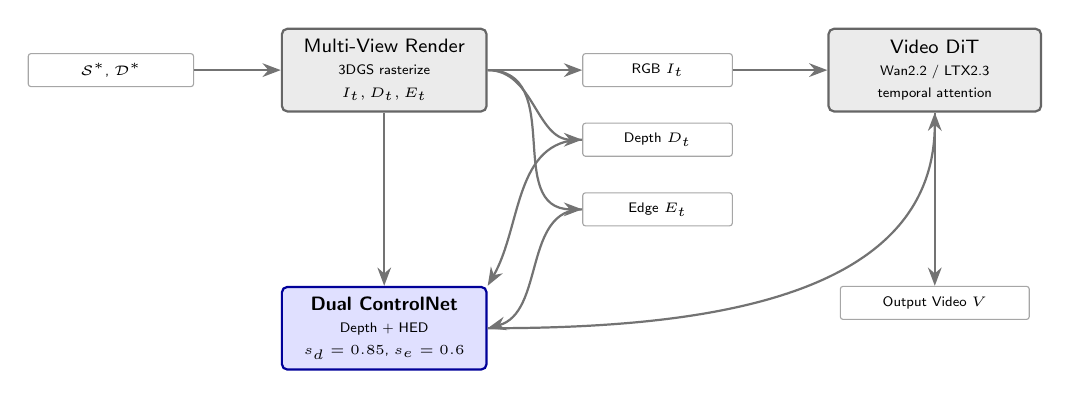
\begin{tikzpicture}[
        font=\sffamily,
        bx/.style={draw=black!60, fill=black!8, rounded corners=2pt,
                   minimum width=2.5cm, minimum height=0.72cm, align=center,
                   font=\sffamily\scriptsize, thick},
        acc/.style={draw=blue!60!black, fill=blue!12, rounded corners=2pt,
                    minimum width=2.5cm, minimum height=0.72cm, align=center,
                    font=\sffamily\scriptsize, thick},
        data/.style={draw=black!35, fill=white, rounded corners=1pt,
                     font=\sffamily\tiny, minimum width=2.1cm,
                     minimum height=0.42cm, align=center},
        ar/.style={->, >=Stealth, thick, draw=black!55}
    ]
        \node[data] (sc) {$\mathcal{S}^*$, $\mathcal{D}^*$};

        \node[bx, right=1.1cm of sc, minimum width=2.6cm,
              minimum height=1.05cm] (rend)
            {Multi-View Render\\{\tiny 3DGS rasterize}\\{\tiny $I_t, D_t, E_t$}};

        \node[data, right=1.2cm of rend, minimum width=1.9cm] (fr) {RGB $I_t$};
        \node[data, below=0.45cm of fr,   minimum width=1.9cm] (df) {Depth $D_t$};
        \node[data, below=0.45cm of df,   minimum width=1.9cm] (ef) {Edge $E_t$};

        \node[acc, below=2.2cm of rend, minimum width=2.6cm,
              minimum height=1.05cm] (cn)
            {\textbf{Dual ControlNet}\\{\tiny Depth + HED}\\{\tiny $s_d=0.85$, $s_e=0.6$}};

        \node[bx, right=1.2cm of fr, minimum width=2.7cm,
              minimum height=1.05cm] (vd)
            {Video DiT\\{\tiny Wan2.2 / LTX2.3}\\{\tiny temporal attention}};

        \node[data, below=2.2cm of vd, minimum width=2.4cm] (out)
            {Output Video $V$};

        \draw[ar] (sc.east)   -- (rend.west);
        \draw[ar] (rend.east) -- (fr.west);
        \draw[ar] (rend.east) to[out=0,in=180,looseness=1.0] (df.west);
        \draw[ar] (rend.east) to[out=0,in=180,looseness=1.2] (ef.west);
        \draw[ar] (fr.east)   -- (vd.west);

        \draw[ar] (rend.south) -- (cn.north);
        \draw[ar] (df.west) to[out=180,in=60,looseness=1.0] (cn.north east);
        \draw[ar] (ef.west) to[out=180,in=15,looseness=1.0] (cn.east);

        \draw[ar] (cn.east) to[out=0,in=-90,looseness=1.0] (vd.south);
        \draw[ar] (vd.south) -- (out.north);
    \end{tikzpicture}}
    \caption{\textbf{ArtiFlow (Variant C).} Grayscale with blue accent on the
    dual-ControlNet conditioning, highlighting the control mechanism.}
    \label{fig:artiflow_C}
\end{figure}


\end{document}
